\documentclass[draft=false]{oblivoir}
\author{Moon Il-chul \\ \href{mailto:icmoon@kaist.ac.kr}{icmoon@kaist.ac.kr} 
   \and Myung Jiyoon \\ \href{mailto:jiyoon9704@kaist.ac.kr}{jiyoon9704@kaist.ac.kr} }
\setcounter{chapter}{18}
\title{Chapter 18. Undirected Probabilistic Graphical Model}
\usepackage{indentfirst}
\usepackage{graphicx}
\usepackage[draft=false]{hyperref}
\usepackage{amsmath}
\usepackage{amssymb}
\usepackage{amsfonts}
\usepackage[]{algorithm2e}
\usepackage{geometry}
\usepackage{algorithm}
\usepackage{algpseudocode}
\hypersetup{pdfborder={0 0 0}}
\renewcommand{\theequation}{\thechapter.\arabic{equation}}
\newlength\myindent
\setlength\myindent{5em}

\begin{document}

\maketitle
\tableofcontents

% 1. -----------------------------------------------------------------
\section{Motivations}

% 1.1 -----------------------------------------------------------------
\subsection{Detour: Bayesian Network}
본격적으로 Undirected Graphical Model(UGM)에 대해 살펴보기 전에 영감을 얻기 위해 Directed Graphical Model(DGM)의 대표적인 예시인 베이지안 네트워크(Bayesian Network)에 대해 다시 짚고 넘어가보자. 
Bayesian Network는 그림 \ref{fig:18-1}과 같이 변수들 사이의 관계를 나타낸 Directed Graphical Model의 일종이다. 이 때 변수들은 확률 변수(Random variable)로서, 각 변수들은 각자의 확률 분포(Probability distribution)을 가지며 이 분포는 매개 변수(Parameter)로 표현된다. 이러한 베이지안 네트워크는 조건부 독립(Conditional independence)을 나타내는데, 이를테면 그림 \ref{fig:18-1}에서는 Y가 주어졌을 때, $X_1$과 $X_2$가 독립인 상황을 보여주고 있다. 종합하자면, 베이지안 네트워크는 구조화된 확률 변수 모델(Structured random variables model)로서 변수들 간의 Full joint distributions을 나타낸다. 베이지안 네트워크를 표현하기 위해서는 directed acyclic graph(DAG), nodes, arcs와 같은 syntax가 사용되는데, 이번 장에서는 이러한 syntax를 따르지 않고 UGM으로 full joint distribution을 나타낼 수 있는 방법에 대해 배울 것이다.

\begin{figure}[ht] \centering 
  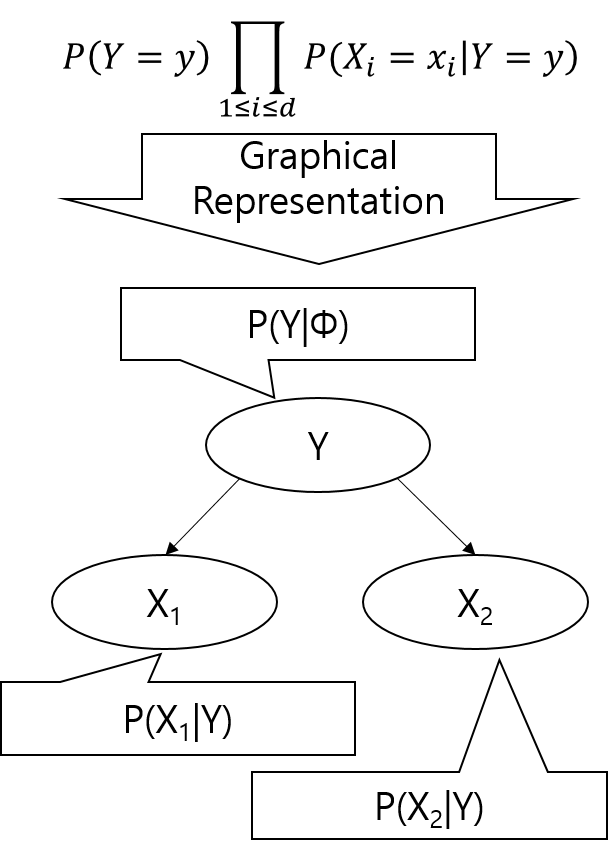
\includegraphics[scale=0.6]{bayesiannetwork.png}
  \caption{Bayesian Network}
  \label{fig:18-1}
\end{figure}

Undirected graphical model로 표현하고자 하는 것을 구체화하기 위해 베이지안 네트워크의 구성요소들을 자세히 살펴보도록 하자. 베이지안 네트워크를 구성하는 요소들은 크게 Qualitative components와 Quantitative components로 나뉘는데, qualitative components로는 변수들 간의 관계구조를 나타내는 casual relationship과 prior knowledge 등이 있고, quantitative components로는 이를 정량적으로 표현하는 조건부 확률 분포(Conditional probability distribution)가 있다. 이 조건부 확률 분포 역시 변수들의 확률 분포와 마찬가지로 paramter로 나타낼 수 있다. 이제 우리는 UGM 조건 하에서 이러한 구성요소들을 어떻게 나타낼 수 있을지 생각해보아야 한다.

% 1.2 -----------------------------------------------------------------
\subsection{Detour: Potential Function}

\begin{figure}[ht] \centering 
  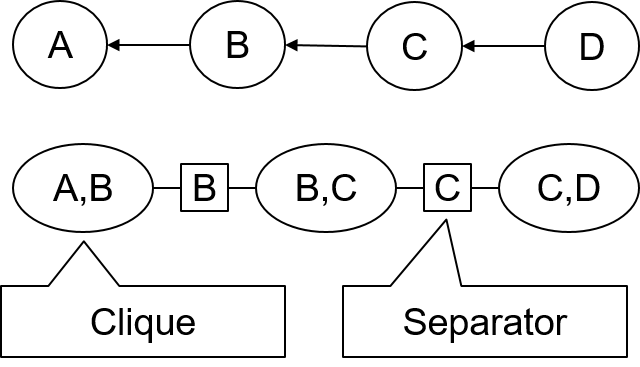
\includegraphics[scale=0.6]{potentialfunction.png}
  \caption{Potential Function}
  \label{fig:18-2}
\end{figure}

이번에는 베이지안 네트워크 장에서 소개했던 Potential Function에 대해 다시 살펴보자. 그림 \ref{fig:18-2}를 보면 이전에 우리가 A,B,C,D로 구성된 베이지안 네트워크를 Clique과 Seperator로 구성된 아래의 구조로 변형시킨 기억을 떠올릴 수 있을 것이다. 이때 아래의 구조는 방향성(direction)이 없기 때문에 potential function은 UGM의 한 일종이라고 할 수 있다. 따라서 potential function 구조에서 변수들 간의 관계를 어떻게 표현했는지 살펴보면 UGM을 구성하기 위한 좋은 motivation으로 삼을 수 있다. Potential function 구조에서 어떻게 함수를 정의했는지는 수식 \ref{eq:18-1}을 참고하길 바란다. 이 식을 참고하여 다음 장에서는 UGM에서 어떻게 변수들 간의 관계를 factorized된 확률 분포 식으로 나타낼 수 있을지 살펴보도록 하자.  
\begin{equation}
P(A,B,C,D) = P(U) = \frac{ \prod_{N} \psi(N) }{ \prod_{L} \phi(L) } = \frac{\psi(A,B)\psi(B,C)\psi(C,D) }{ \phi(B) \phi(C) }
\label{eq:18-1}
\end{equation} 


% 2. -----------------------------------------------------------------
\section{Markov Random Field}

% 2.1 -----------------------------------------------------------------
\subsection{Undirected Graphical Model}

\begin{figure}[ht] \centering 
  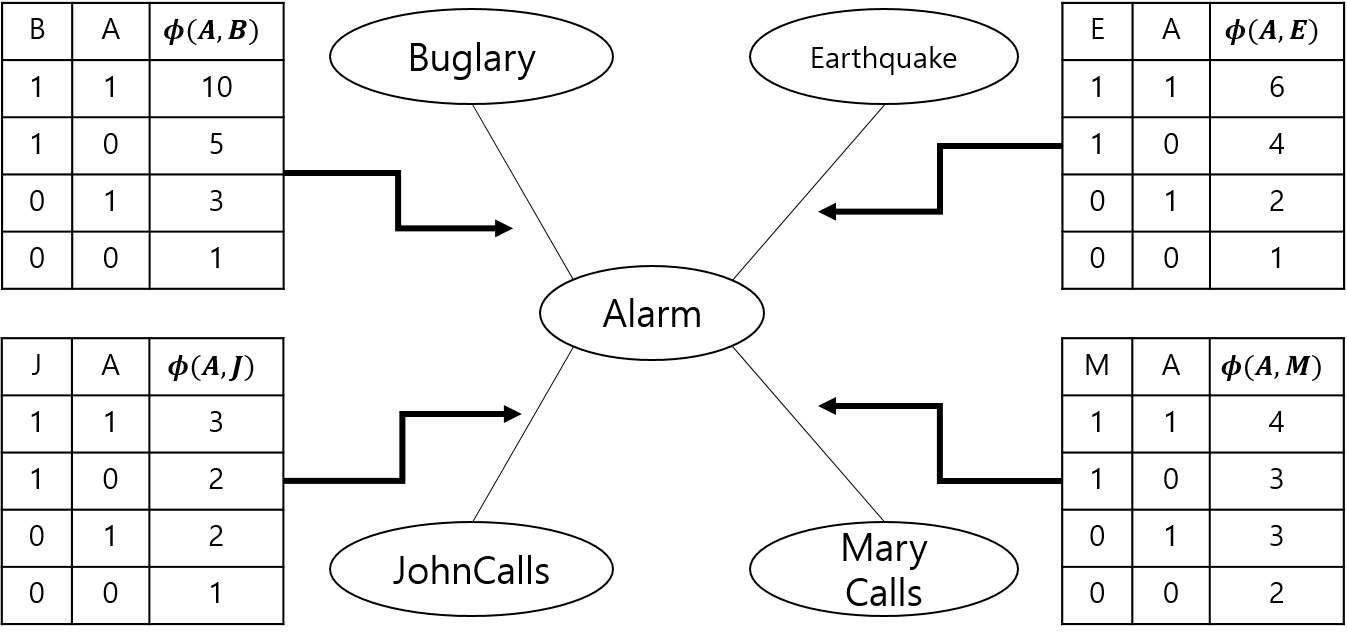
\includegraphics[scale=0.6]{UGM.png}
  \caption{Example of Undirected Graphical Model}
  \label{fig:18-3}
\end{figure}

이제 본격적으로 UGM 구조를 살펴보도록 하자. DGM과 쉽게 비교하기 위해 앞에서 살펴보았던 Alarm 예제를 UGM 구조로 다시 나타내었다(그림 \ref{fig:18-3}). 기존의 DGM 구조에서는 방향성이 존재했기 때문에 변수들 간의 관계를 $P(A\mid B)$와 같은 조건부 확률로 나타내었지만 UGM에서는 방향성이 존재하지 않기 때문에 이처럼 나타낼 수 없다. 때문에 UGM에서는 조건부 확률 대신에 $\phi(A,B)$와 같은 potential function을 정의한다. 이 potential function은 두 변수를 잇는 edge에 정의하는데, 각 변수의 instance에 따른 score 값을 부여한다. 이 score 값은 normalize되어 있지 않으므로 이 값 자체를 확률로 볼 수는 없지만 joint probability가 될 수 있는 잠재성(potential)이 있는 값이다. 즉, 변수들로 이루어진 특정 event의 likelihood를 measure하는 값이다. 그 예시로 그림 \ref{fig:18-3}은, B가 1이고 A가 1일 가능성은 10점으로 scoring하고 B가 1이고 A가 0일 가능성은 5점으로 scoring한 경우이다. 더불어, 이러한 potential function은 모델의 전체 구조를 명시해주고 있는데, 예를 들어 그림 \ref{fig:18-3}에서 Buglary와 Alarm의 dependency를 $\phi(A,B)$이 나타내주고 있고 반면 Buglary와 Earthquake는 관련성이 없기 때문에 변수 사이의 edge와 potential function이 정의되지 않은 것을 볼 수 있다. 

이제 정의한 potential function들로 전체 모델의 full joint distribution을 정의하기 위해서는 각 edge에 부여된 potential function을 모두 곱하고, 모든 가능성에 대하여 더해준 normalizing constant $z$로 나누어주면 된다(수식 \ref{eq:18-2}). 즉 UGM에서는 변수들 사이에 정의한 potential function(scoring mechanism)을 확률 모델로 만들어내는 구조라고 볼 수 있다.

\begin{equation}
	P(B,E,A,J,M) = {\phi(A,B)\phi(A,E)\phi(A,J)\phi(A,M) \over \sum_{A,B,E,J,M}\phi(A,B)\phi(A,E)\phi(A,J)\phi(A,M)}
\label{eq:18-2}
\end{equation}

% 2.2 -----------------------------------------------------------------
\subsection{Markov Random Field}
이번 절에서는 앞서 소개한 UGM의 구체적인 예시인 Markov Random Field에 대해 알아보도록 하자. Markov Random Field란 UGM에서 정의된 변수들 간의 관계를 나타낸 probabilistic distribution, 즉 변수들의 full joint distribution을 의미한다. 이 distribution을 수식으로 나타내면 수식 \ref{eq:18-3}와 같다. 

\begin{equation}
	p(x_1,\dots, x_n) = {1 \over Z}\prod_{c\in C}\phi_c(x_c)
\label{eq:18-3}
\end{equation}

수식 \ref{eq:18-3}는 $C$라는 notation외에는 수식 \ref{eq:18-2}과 같은 형식인데, 이때 이 $C$는 전체 모델에 있는 Clique, 즉 completely connected subgraph를 의미한다. 예를 들어 그림 \ref{fig:18-4}를 보면, 왼쪽의 구조는 모든 변수가 연결되어 있기 때문에 clique가 되지만 오른쪽의 구조는 B와 D가 연결되어 있지 않으므로 clique가 될 수 없다. 즉, 수식 \ref{eq:18-3}의 우변은 전체 UGM 구조에 있는 maximal cliques에 대해서 potential function을 곱해준 뒤 normalizing constant로 나눠준 식이다. 이 때, edge는 가장 작은 단위의 clique이기 때문에 수식 \ref{eq:18-2}은 모든 maximal clique가 edge인 경우를 나타낸다. 그러나 만약 그림 \ref{fig:18-3}에서 Buglary와 Earthquake도 연결되어 있었다면, A,B,E를 잇는 삼각형이 maximal clique이기 때문에 $\phi(A,B)$와 $\phi(A,E)$ 대신 $\phi(A,B,E)$로 표현해야 한다. 

\begin{figure}[ht] \centering 
  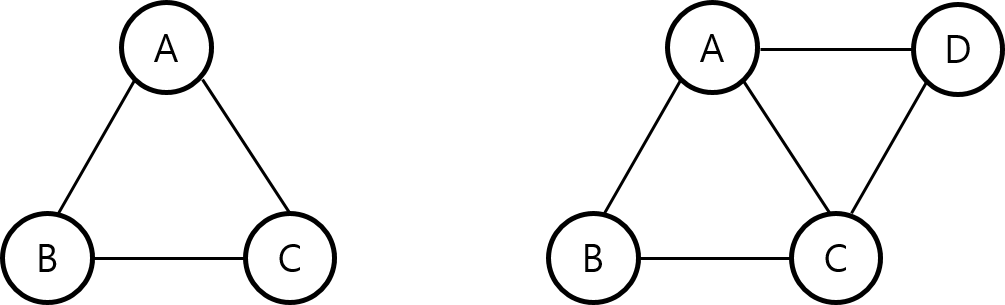
\includegraphics[scale=0.6]{clique.png}
  \caption{Example of Clique(left) and non-Clique(right) Structure}
  \label{fig:18-4}
\end{figure}



다음으로, potential function $\phi_c$는 각 clique의 변수들로 정의된 nonnegative funtion이다. 즉 scoring 값으로 음수는 정의할 수 없다. 마지막으로, 수식 \ref{eq:18-3}의 분모가 각 변수가 특정 값으로 instantiate된 경우의 potential function을 곱해준 값이라면, normalizing constant Z는 모든 가능한 경우에 대해 이를 더해준 값이다(수식 \ref{eq:18-4}). 이 때, clique의 개수와 발생 가능한 combination이 많으면 $Z$를 계산하는 것 자체도 상당한 일이다.
\begin{equation}
	Z = \sum_{x_1\dots x_n}\prod_{c\in C}\phi_c(x_c)
\label{eq:18-4}
\end{equation}

% 3. -----------------------------------------------------------------
\section{Conditional Random Field}

% 3.1 -----------------------------------------------------------------
\subsection{Comparison of MRF and CRF}
앞서 배운 Markov Random Field(MRF)의 inference 과정을 자세히 살펴보기 전에 MRF보다 좀 더 다루기 쉬운 Conditional Random Field(CRF)에 대해 먼저 알아보자. 

\begin{figure}[ht] \centering 
  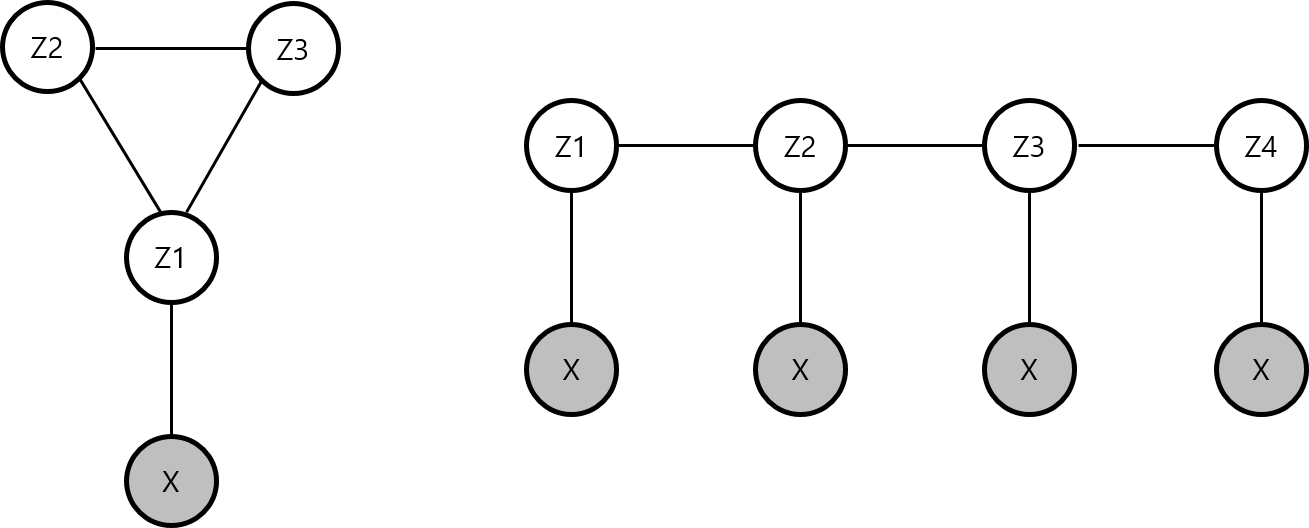
\includegraphics[scale=0.6]{MRFCRF.png}
  \caption{Example of MRF(left) and CRF(right) Structure}
  \label{fig:18-5}
\end{figure}

그림 \ref{fig:18-5}의 왼쪽 구조는 기본 MRF 구조, 오른쪽은 CRF 구조의 예시로서  X는 observed variable, Z는 latent variable을 나타낸다. 먼저 MRF 구조에서는 Z에 assignment를 부여하기 위해서 likelihood $P(X,Z)$를 maximize하기 때문에 이는 unsupervised 과정이다. 반면, 오른쪽의 CRF 구조에서는 X가 주어진 상황에서 conditional probability $P(Z\mid X)$를 maximize하기 때문에 supervised 과정이라고 할 수 있다. 이 때, supervised method가 unsupervised method에 비해 간단하고 이해하기 쉽기 때문에 우리는 CRF에 대해 배운 뒤에 MRF를 본격적으로 배우도록 하겠다. 

% 3.2 -----------------------------------------------------------------
\subsection{Limitations of Hidden Markov Model}
그림 \ref{fig:18-5}의 오른쪽에 있는 CRF 구조를 살펴보면 우리가 앞서 배운 Hidden Markov Model(HMM)과 아주 유사한 구조라는 것을 알 수 있다. 따라서 이번 절에서는 HMM을 review함과 동시에 HMM의 한계에 대해 짚고 넘어가보자. 

\begin{figure}[ht] \centering 
  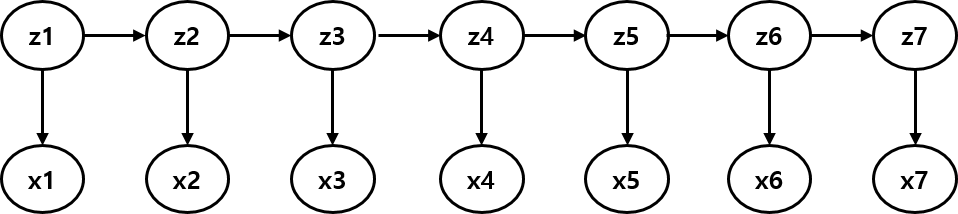
\includegraphics[scale=0.6]{hmm.png}
  \caption{Structure of Hidden Markov Model}
  \label{fig:18-6}
\end{figure}

먼저, HMM에서 현재의 state는 현재의 observation과만 직접적으로 영향을 주고받는다. 물론, latent variable Z가 propagate하는 과정에서 이전 단계의 Z와 이후 단계의 Z와 연결점을 가지지만 이 때의 observation과는 직접적으로 연결되어 있지 않다. 예를 들어, 그림 \ref{fig:18-6}에서 보면 Z2가 X2와는 연결되어 있지만 X1, X3과는 직접적으로 연결되어 있지 않은 것을 볼 수 있다. 이 때의 문제점을 생각해보자. ``나는 밥을 먹는다." 라고 하는 자연어에서 `밥을'의 품사를 추론한다고 할 때, `밥을'이 목적어라는 것을 유추할 때에 분명히 `나는'이라는 주어와 `먹는다'라는 서술어의 존재가 큰 영향을 미칠 것임에도 불구하고 HMM에서는 이 관계를 모델링할 수 없다.  

둘째로, Z의 propagate 과정에서 앞에있는 Z가 이후의 Z에는 영향을 미치지만 그 반대로는 영향을 미치지 못한다. 즉, HMM에서는 forward dependencies만 존재한다. 이 경우에도 마찬가지로 ``나는 밥을 먹는다." 에서 `나는'의 존재가 `밥을'이라는 목적어의 존재의 영향을 받는 데도 불구하고 이를 모델링할 수 없는 문제가 생긴다. 

마지막으로, HMM은 generative model의 일종으로서, classification task에 사용하기에는 좋은 모델이 아니다. HMM은 Z를 assign할 때에 likelihood $P(X,Z)$를 maximize하는데, classification task에서 우리의 본 목적은 $P(Z\mid X)$를 maximize하는 Z를 찾는 것이기 때문에 방식의 차이가 있다. 수식 \ref{eq:18-5}를 참고하면 HMM에서 $P(X,Z)$를 optimize한다는 것은 $P(X\mid Z)P(Z)$ 즉, HMM에서 emission과 Z의 propagation을 각각 모델링하여 이를 optimize하겠다는 것인데, classification task에서는 굳이 이렇게 하지 않고 $P(Z\mid X)$ 자체를 모델링하는 것이 더 효율적인 방법이다. 따라서 이후의 장에서 우리는 CRF가 $P(Z\mid X)$를 직접 모델링하는 방법에 대해 배울 것이다. 

\begin{equation}
	P(Z\mid X) = {P(X,Z) \over P(X)} = {P(X\mid Z)P(Z) \over P(X)}
\label{eq:18-5}
\end{equation}


% 3.3 -----------------------------------------------------------------
\subsection{Alternative: Maximum Entropy Markov Model}
이번 절에서는 CMF와 비슷하게 $P(Z\mid X)$을 직접 모델링하는 discriminative model 중 하나인 Maxmimum Entropy Markov Model(MEMM)에 대해 알아보도록 하자. 

\begin{figure}[ht] \centering 
  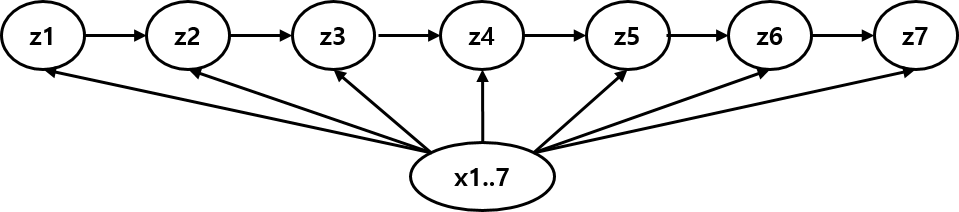
\includegraphics[scale=0.6]{memm.png}
  \caption{Structure of Maximum Entropy Markov Model}
  \label{fig:18-7}
\end{figure}
\begin{equation}
	P(Z_{1:n}\mid X_{1:n}) = \prod_{i=1}^n {P(z_i\mid z_{i-1},X_{1:n}}) =  \prod_{i=1}^n {exp(w^T f(z_i,z_{i-1},X_{1:n})) \over \sum_{z_j} {exp(w^T f(z_j,z_{i-1},X_{1:n}))}} = \prod_{i=1}^n {exp(w^T f(z_i,z_{i-1},X_{1:n})) \over Z(z_{i-1}, X_{1:n})}
\label{eq:18-6}
\end{equation}

그림 \ref{fig:18-7}을 보면 HMM과는 달리 화살표 방향이 X에서 Z로 향하는 것을 볼 수 있다. 즉 MEMM에서는 $P(X\mid Z)$를 모델링하는 것이 아닌 $P(Z\mid X)$를 직접 모델링한다. 이 때, $z_i$가 $z_{i-1}$과 $x_{1:n}$로부터 영향을 받는 구조가 수식 \ref{eq:18-6}의 첫번째 등식에 나타나 있다. 이 때 이 두번째 식은 logistic regression에서 보았던 식과 유사한 형태를 띠고 있다(수식 \ref{eq:18-7}). 따라서, logistic regression에서 모델링한 것과 비슷하게 MEMM에서도 두번째 등식과 같이 모델링할 수 있다. 이때 이 식은 softmax의 형태를 띠고 있다. 여기서 $f$란 feature function으로서 $Z_{i-1}$, $Z_i$, $X$를 인풋으로 받아서 feature을 뽑아내는 역할을 한다. 이 때 이 function은 도메인에 따라 모델러가 직접 정의하는 함수이다. 이제 MEMM에서 우리가 추론하고자 하는 파라미터는 $w$인데, 이를 추론하는 과정은 logistic regression 모델과 마찬가지로 gradient descent method를 통해 $P(Z\mid X)$를 maximize하는 $w$를 찾아주면 된다. 이제 우리의 본 목적은 MEMM을 CRF로 만들어 주는 것인데, 그러기 위해서는 feature function $f$를 potential function $\phi$로 바꾸어주면 된다. 이에 대해서는 다음 절에서 자세히 살펴보도록 하자. 
\begin{equation}
	P(Y\mid X) = {1 \over e^{-W X}+1} = {e^{W X} \over e^{W X }+1}
\label{eq:18-7}
\end{equation}

% 3.4 -----------------------------------------------------------------
\subsection{Conditional Random Field}
앞서 알아본 MEMM 모델을 토대로 이번 절에서는 Conditional Random Field(CRF) 모델에 대해 본격적으로 알아보자. CRF 모델은 Undirected Graph Model의 일종이기 때문에 MEMM 구조와 유사하지만 방향성이 없는 구조를 가진다(그림 \ref{fig:18-8}).  CRF 역시 MEMM과 마찬가지로 conditional probability $P(Y\mid X)$를 모델링하지만 방향성이 없기 때문에 $P(y_i\mid y_{i-1},X)$ 대신에 potential function $\phi$로 표현된다(수식 \ref{eq:18-8}). 이 수식은 normalizing constant $Z$와 각 clique들의 potential function의 곱으로 이루어져 있어 전형적 MRF의 수식(\ref{eq:18-3})과 같은 형태를 띠고 있다. (여기서 우리는 CRF 구조 속의 존재하는 maximal clique가 $(y_i,y_{i-1},X_{1;n})$임을 쉽게 알 수 있다.) 이 때 potential function $\phi$의 형태를 어떻게 모델링하는 지는 수식 \ref{eq:18-8}의 두번째 줄에 나타나 있다. 이를 보면 exponential function을 통해 scoring의  nonnegativity가 보장되고 potential function간의 $\prod$(product)로 되어 있던 부분이 exp 안에서 $\sum$(sum)형태로 바뀐 것을 볼 수 있다. 여기서 $f_k$와 $g_k$는 모두 feature function으로서 직접적으로 명시되어 있지는 않지만 $f$는 $y_{i-1}$로부터 $y_i$가 propagation되는 과정을, $g$는 $y_i$로부터 $X$가 emission되는 과정에 scoring mechanism을 부여한 것이다. 이 때 $f$의 경우 k개 만큼의, $g$의 경우 $l$개 만큼의 다양한 scoring이 존재할 수 있음을 나타낸다. 또한, MEMM의 파라미터가 $w$였다면, CRF의 파라미터는 $\lambda$와 $\mu$로, 이 둘을 통해 각 feature들의 중요도가 정해진다. 결론적으로, CRF 모델은 Bayesian Network처럼 Propagtion과 Emission 과정을 직접적으로 probabilistic modeling하고 있지는 않지만, 각 clique의 potential function을 scoring함으로써 그 과정을 어느정도 나타내고 있다.

\begin{figure}[ht] \centering 
  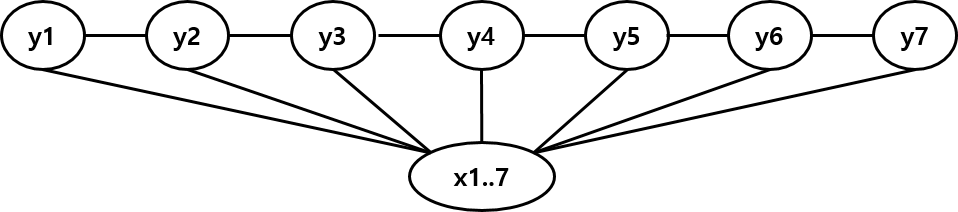
\includegraphics[scale=0.6]{CRF.png}
  \caption{Structure of Conditional Random Field Model}
  \label{fig:18-8}
\end{figure}

\begin{gather}
	P(Y_{1:n}\mid X_{1:n}) = {1 \over Z(\lambda,\mu,X_{1:n})} \prod_{i=1}^{n}{\phi(y_i,y_{i-1},X_{1:n})}\nonumber\\
	={1 \over Z(\lambda,\mu,X_{1:n})}exp(\sum_{i=1}^{n}(\sum_k\lambda_k f_k(y_i,y_{i-1},X_{1:n})+\sum_l{\mu_k g_l(y_i,X_{1:n})}))
\label{eq:18-8}
\end{gather}

\begin{equation}
	Z(\lambda,\mu,X_{1:n})=\sum_{Y_1:n}exp(\sum_{i=1}^{n}(\sum_k\lambda_k f_k(y_i,y_{i-1},X_{1:n})+\sum_l{\mu_k g_l(y_i,X_{1:n})}))
\label{eq:18-9}
\end{equation}

% 3.5 -----------------------------------------------------------------
\subsection{Logistic Regression and Conditional Random Field}
우리는 이전에 generative-discriminative pairs에 대해 배운 적이 있다. 우선 generative model과 discriminative model의 정의를 다시 짚고 넘어가자면, $P(Y\mid X)$를 모델하기 위해 generative model에서는 $P(X\mid Y)P(Y)$를 각각 모델하여 이를 유도하는 반면, discriminative model에서는 $P(Y\mid X)$자체를 모델링한다. 이에 서로 counter part로 작용하는 generative model-discriminative pairs가 존재하는데 Naive Bayes Classifier와 Logistic Regression(LR)이 그 대표적인 예시이다. 또한, 우리가 이번 장에서 배운 HMM과 CRF도 sequence model로써의  generative-discriminative pair를 형성한다. 따라서 이번 절에서는 discriminative model의 예시인 LR과 CRF의 공통점을 알아보고자 한다.

물론 기본적으로 LR과 CRF는 다른 목적을 가지는 모델이다. LR은 instance중심의 데이터를, CRF는 temporal data를 다루는 모델이기 때문이다. 그러나 두 모델 모두 discriminative model이기 때문에 파라미터를 inference하는 과정에는 유사함이 있다. 
본격적으로 LR과 CRF를 비교하기 위해 우리는 몇가지 가정을 하고자 한다. 첫째로, CRF 모델과 달리 LR에서의 Y는 하나의 instance이기 때문에 Y의 dimension을 single dimension로 고정한다. 즉 $Y_{1:n}$이 아닌 $Y_1$만 존재한다고 가정한다. 둘째로, $X_{1:n}$를 간단히 하기 위해 각 $X_i$를 binary variable로 가정한다. 마지막으로, CRF의 feature function $f$와 $g$를 indicator function $\mathbbm{1}_{X_i=1, Y=1}$로 가정한다. 
수식 관점에서 보면, $Y$가 더이상 temporal data가 아닌 하나의 instance이기 때문에 propagation을 나타내는 featuren function $f$ 부분이 사라지고, normalizing constant $Z$도 두가지 경우의 합으로 specify할 수 있다. 그 식을 정리하면, 수식 \ref{eq:18-10}과 같다. 마지막 식을 보면, logistic function 속의 X의 linear combination이 들어간 형태로써 전형적인 LR의 식을 띠고 있다. 이로써 우리는 CRF와 LR의 유사성을 증명하였다.  따라서, 우리가 LR에서 Gradient Descent Method를 통해 파라미터 $\theta$를 inference했던 방법을 이용해 CRF에서도 파라미터를 inference할 수 있다.  

\begin{gather}
	P(Y=1\mid X_{1:n}) = {1 \over Z(\lambda,\mu,X_{1:n})} exp(\sum_{i=1}^n{\lambda_k\mathbbm{1}_{X_i=1, Y=1} }) \nonumber\\
    = {exp(\sum_{i=1}^n \lambda_k\mathbbm{1}_{X_i=1, Y=1} ) \over {exp(\sum_{i=1}^n{\lambda_k\mathbbm{1}_{X_i=1, Y=0} })+exp(\sum_{i=1}^n{\lambda_k\mathbbm{1}_{X_i=1, Y=1} })}}\nonumber\\
	= {exp(\sum_{i=1}^n\lambda_k X_i) \over exp(0)+exp(\sum_{i=1}^n\lambda_k X_i)}	= {1 \over exp(\sum_{i=1}^n-\lambda_k X_i)+1}
\label{eq:18-10}
\end{gather}

% 3.6 -----------------------------------------------------------------
\subsection{Parameter Inference of Conditional Random Field}
앞서 우리는 CRF과 LR과 유사한 형태를 띠고 있어 CRF도 LR과 같이 Gradient Descent Method로 parameter inference를 수행할 수 있다는 것을 배웠다. 그러기 위해서는 우선 $P(Y\mid X)$의 gradient를 구해야 한다. 그런데 수식 \ref{eq:18-9}을 보면, normalizing constant $Z$는 모든 데이터에 대한 합의 형태를 띠고 있기 때문에 $Z$의 gradient를 구하는 것은 그리 간단하지 않은 일이다. 따라서 $Z$의 gradient를 쉽게 구하기 위해 이전에 배웠던 Exponential Family에 대해 다시 짚고 넘어가고자 한다. 

Exponential family란 변수 $x$의 probability density function(pdf)를 수식 \ref{eq:18-11}과 같이 나타낼 수 있는 경우를 말한다. 여기서 $T(x)$는 sufficient statistics, $\eta(\theta)$는 natural parameter, $A(\theta)$는 log normalizer라고 부른다. 이때 log normalizer $A(\theta)$에 주목해보면, 이 식은 CRF의 수식 \ref{eq:18-8}에서 ${1 \over Z(\lambda,\mu,X_{1:n})}$에 log를 취한 후 $exp$ 부분 안으로 넣어주었을 때와 같은 형태를 띠고 있는 것을 알 수 있다. 또한, 수식 \ref{eq:18-8}의 $exp$ 안쪽 부분은 parameter인 $\mu,\lambda$와($\eta(\theta)$) 데이터와 연관된 $f_k,g_k$로($T(x)$)의 linear combination으 이루어져 있기 때문에 수식 \ref{eq:18-8}전체를 exponential family와 같은 형태로 나타낼 수 있다. 

\begin{equation}
	P(x\mid \theta) = h(x) exp(\eta(\theta) T(x)-A(\theta))
\label{eq:18-11}
\end{equation}

앞서 우리는 exponential family에서 log normalizer의 derivative가 sufficient statistics의 moment임을 배운 바가 있다(수식 \ref{eq:18-12}). 이제는 우리가 CRF의 식이 exponential family의 형태이고 normalizing constant $Z$가 log normalizer의 역할을 한다는 것을 알기 때문에 sufficient statistics $T(x)$의 평균을 구함으로써 $Z$의 gradient를 구할 수 있다.
\begin{eqnarray}
\frac{d}{d\eta}A(\eta)  = 
\frac{d}{d\eta}log\int h(x)exp\{\eta^{T}T(x)\}dx = \frac{\int T(x)h(x)exp\{\eta^{T}T(x)\}dx}{\int h(x)exp\{\eta^{T}T(x)\}dx}\nonumber\\
 =  \frac{\int T(x)h(x)exp\{\eta^{T}T(x)\}dx}{exp(A(\eta))}=\int T(x)h(x)exp\{\eta^{T}T(x)-A(\eta)\}dx = E_{p}|T(x)|\nonumber\\
\label{eq:18-12}
\end{eqnarray}

이제 본격적으로 CRF의 parameter를 inference하는 과정에 대해 살펴보자. 데이터 $X,Y$가 주어지는 supervised learning하에서는 데이터의 likelihood를 maximize하는 MLE방법으로 parameter를 inference하는 것이 일반적이다. CRF에서의 likelihood는 전체 데이터에 대한 $P(Y\mid X)$의 곱으로, $P(Y\mid X)$는 수식 \ref{eq:18-8}과 같이 나타낼 수 있다. 이때 전체식에 log를 취해주면 $exp$ 안의 부분이 sum 형태로 바뀌어 나오게 되고 normalizing constant $Z$는 $-log Z$의 형태로 바꿀 수 있다(수식 \ref{eq:18-13}).
여기서 한가지 주의할 점은, 그동안 constant라고 불리는 값은 optimization을 할 때 제외하고 고려해왔지만 여기의 normalizing constant $Z$는 다르다. $Z$ 또한 명백히 우리가 얻고자 하는 $\lambda$ 와 $\mu$에 대한 함수이기 때문에 gradient를 구할 때 $Z$를 제외해서는 안된다. 따라서 우리는 수식 \ref{eq:18-13} 전체를 고려해서 parameter inference를 수행해야 한다. 


\begin{gather}
    \lambda^*,\mu^* = argmax_{\lambda,\mu}L(\lambda,\mu) = argmax_{\lambda,\mu} {\prod_{d\in D}P(Y_{d,1:n}\mid X_{d,1:n};\lambda,\mu)} \nonumber \\
    = argmax_{\lambda,\mu}{\prod_{d\in D} 
	{1 \over Z(\lambda,\mu,X_{1:n})}exp(\sum_{i=1}^{n}(\sum_k\lambda_k f_k(y_{d,i},y_{d,i-1},X_{d,1:n})+\sum_l{\mu_k g_l(y_{d,i},X_{d,1:n})}))} \nonumber \\
	= argmax_{\lambda,\mu}{\sum_{d\in D}[\sum_{i=1}^n(\sum_k\lambda_k f_k(y_{d,i},y_{d,i-1},X_{d,1:n})+\sum_l{\mu_k g_l(y_{d,i},X_{d,1:n})})-log Z(\lambda,\mu,X_{d,1:n})]}
\label{eq:18-13}
\end{gather}

이제 수식 \ref{eq:18-13}의 gradient를 구해서 parameter를 inference하는 과정을 살펴보자. $\lambda$와 $\mu$ 각각에 대해 gradient를 구해서 $\lambda^*, \mu^*$를 찾아야 하지만 두 과정이 거의 동일하기 때문에 여기에서는 $\lambda$에 대한 optimize 과정만 살펴보겠다. 우선 $\lambda_k$에 대한 likelihood(수식 \ref{eq:18-13})의 gradient를 구하면, $\lambda$와 관련이 없는 $g_l$에 대한 식이 사라지고 $\sum_k$에 대한 부분도 사라지므로 수식 \ref{eq:18-14}와 같이 나타낼 수 있다. 이때, ${d\over d_{\lambda_k}} logZ$는 앞서 말한 것 처럼 sufficient statistics의 mean으로 구할 수 있으므로 수식 \ref{eq:18-15}와 같이 표현할 수 있다. 따라서 수식을 모두 정리하면 수식 \ref{eq:18-16}과 같다. 여기서 $Y_{d,1:n}$은 사실 이웃한 $y$끼리의 정보만 사용되기 때문에  $\sum_{Y_{d,1:n}}$이 $\sum_{y_{d,i},y_{d,i-1}}$으로 치환된 것을 볼 수 있다.

\begin{equation}
    \nabla_{\lambda_k}L(\lambda,\mu) = {\sum_{d\in D}[\sum_i^n f_k(y_{d,i},y_{d,i-1},X_{d,1:n})-{d\over d_{\lambda_k}}log Z(\lambda,\mu,X_{d,1:n})] }
\label{eq:18-14}   
\end{equation}

\begin{equation}
    {d\over d_{\lambda_k}}log Z(\lambda,\mu,X_{d,1:n}) = E_{P(Y_{d,1:n}\mid X_{d,1:n};\lambda,\mu)}[\sum_{i=1}^n\sum_k f_k(y_{d,i},y_{d,i-1},X_{d,1:n})]
\label{eq:18-15}   
\end{equation}

\begin{gather}
    \nabla_{\lambda_k}L(\lambda,\mu) = {\sum_{d\in D}[\sum_i^n f_k(y_{d,i},y_{d,i-1},X_{d,1:n}) - \sum_{Y_{d,1:n}}P(Y_{d,1:n}\mid X_{d,1:n};\lambda,\mu)\sum_{i=1}^n\sum_k f_k(y_{d,i},y_{d,i-1},X_{d,1:n})] } \nonumber \\
    = {\sum_{d\in D}[\sum_i^n f_k(y_{d,i},y_{d,i-1},X_{d,1:n}) - \sum_{i=1}^n \sum_{y_{d,i},y_{d,i-1}} \sum_k P(Y_{d,1:n}\mid X_{d,1:n};\lambda,\mu) f_k(y_{d,i},y_{d,i-1},X_{d,1:n})] }
\label{eq:18-16}   
\end{gather}

% 3.7 -----------------------------------------------------------------
\subsection{Neural Network and Conditional Random Field}
이번 절에서는 앞서 배운 CRF의 성질을 바탕으로 Neural Network(NN)에 CRF가 활용될 수 있는 방법에 대해 알아보고자 한다. 기본적으로 NN과 CRF는 유사점이 많다. 앞서 CRF가 특정한 가정 하에서 Logistic Regression으로 변환될 수 있다는 것을 알아본 적이 있는데, 이때 LR은 activiation으로 logistic function을 사용하는 neuron의 대표적인 예시이다. 또한, NN과 CRF 모두 gradient descent를 통해 parameter을 inference한다. 따라서 이 두 모델을 어떻게 상호적으로 운용할 수 있는지 알아보도록 하자. 

\begin{figure}[ht] \centering 
  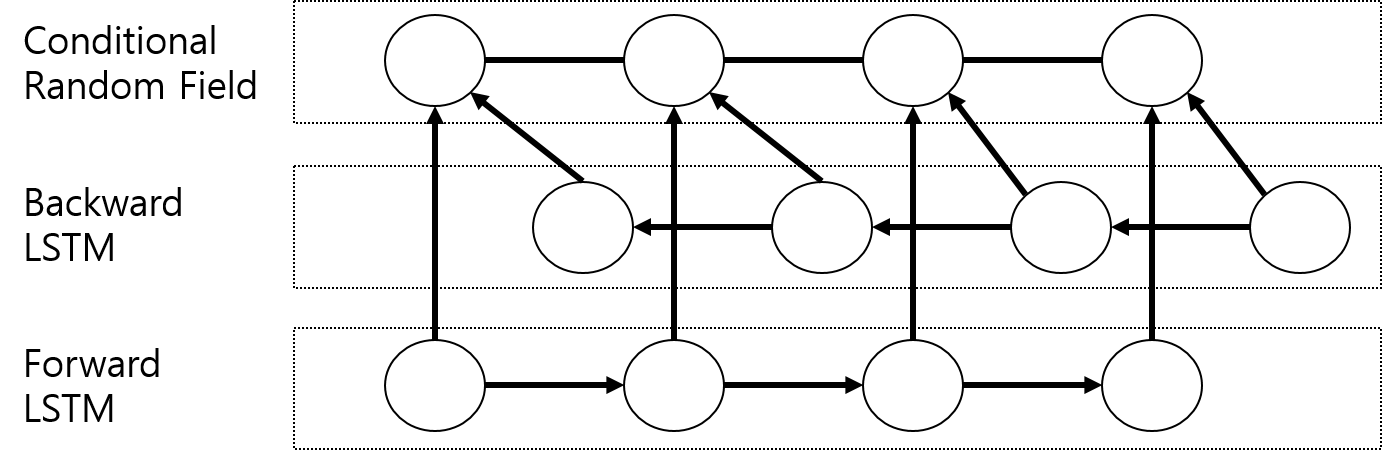
\includegraphics[scale=0.6] {NNCRF.png}
  \caption{Relationship of Neural Network and Conditional Random Field}
  \label{fig:18-9}
\end{figure}

RNN이라고 불리는 Recurrent Neural Network 모델에서는 그림  \ref{fig:18-9}과 같이 시계열 데이터를 모델링한다. 기본적으로 NN은 feed-forward와 back-propagation을 통해 parameter을 learning하기 때문에 방향성이 항상 존재한다. 특히, Natural Language Processing(NLP)와 같이 데이터가 양방향으로 흐르는 모델의 경우 그림 \ref{fig:18-9}와 같은 bidirectional model을 사용한다. 이 때 두 방향의 hidden 데이터를 모아 prediction을 할 때 prediction 간의 connenction을 무시하고 $P(y_1\mid h_{f_1},h_{b_1}), P(y_2\mid h_{f_2},h_{b_2}), \dots$와 같이 개별적으로 모델링하는 경우와 prediction을 종합적으로 고려하여 $P(Y_{1:T}\mid h_{f_{1:T}}, h_{b_{1:T}})$ 전체를 모델링하는 경우가 있다. 이때 후자의 경우 전후의 assignment를 고려해서 prediction을 하기 때문에 더 많은 정보를 활용할 수 있으나 문제점은 NN에서는 방향성이 없는 vector 형태의 $Y_{1:T}$을 모델링하기 힘들다는 점이다. 따라서 여기에서 CRF가 활용될 수 있다. 모델링하고자 하는 $P(Y_{1:T}\mid h_{f_{1:T}}, h_{b_{1:T}})$의 형태는 앞서 배웠던 CRF의 $P(Y_{1:n}\mid X_{1:n})$형태와 동일다(수식 \ref{eq:18-8}). 따라서 우리는 bidirectional RNN 모델의 prediction 파트에서 hidden layer의 정보를 모아 temporal assignment를 할 때 CRF를 활용할 수 있다. 
즉 우리는 Neural Network와 Undirected Graphical Model이 함께 사용될 수 있는 예시에 대해 알아보았다. 
\end{document}
